%!TEX root = thesis.tex

\chapter{Gesture recognition}
\label{ch:gestures}

Knowing the location the hands in a image doesn't tell much about the hand poses. A method needs to be constructed to discriminate the different hand poses. 

This chapter describes how the hand poses are extracted from the hand windows. First features of the hand window are extracted that represent the current hand pose. Then these features are compared by a classifier with previously extracted features of hand poses for which the poses where already known. The classifier will determine which known hand pose(s) resembles the at that moment classified hand.


\section{Feature extraction}
To compare two or more hands with each other a method is required to calculate the similarity. A very simple method is to compare each pixel location with each other and sum all the differences. But there are some problems with this method. First of all, it is not going to work on images that are not the same size or orientation. Also it is computationally expensive for larger images, for an image of 100 by 100 pixels there are already 10.000 dimensions. And a other important thing, this method is not very forgiving for small variations like scaling and rotation.

\subsection*{Segmentation - removing background}


\begin{figure}[htbp]
\begin{center}
\subfloat[Hand window]{
        
\includegraphics[width=0.2\linewidth]{figures/pipeline/lefthand.jpg}
        \label{fig:lefthandwindow}
}
\hspace{0.03\linewidth}
\subfloat[Hand cutout]{
        
\includegraphics[width=0.2\linewidth]{figures/pipeline/lefthandcutout.jpg}
        \label{fig:lefthandcutout}
}
\hspace{0.03\linewidth}
\subfloat[Hand features]{
        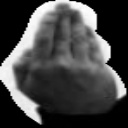
\includegraphics[width=0.2\linewidth]{figures/pipeline/lefthandhog.jpg}
        \label{fig:lefthandfeatures}
}
\end{center}
\end{figure}

The hand window contains some background pixels, because a hand will never fill a perfect square. These pixels are unwanted since they contain arbitrary values that introduce noise into our process. In \autoref{sec:skinmodel} a binary mask for skin pixels is constructed. The binary inversion of this mask can be used again to remove the background.

Sometimes the blob is too small to say something useful about the hand pose. One way to artificially increase the blob size is to do a morphological dilate operation on the blob. This will increase the size of the hand cutout and probably add skin pixels, but this will also introduce more noisy (non-skin) pixels.

\subsection*{Descriptors}
To reduce the number of dimensions of an image a descriptor can be used. A descriptor describes an image in, if properly used, less dimensions than the image itself. Also it can introduce some useful properties like scale an rotation invariance. In this paper only 2 descriptors are discussed, Histogram of oriented gradient\cite{NavneetDalal2006} (HOG) and Speeded Up Robust Features\cite{Bay2006} (SURF).

The HOG descriptor has been successfully applied and studied in human detection \cite{NavneetDalal2006, watanabe2009}. The HOG descriptors method uses a dense grid of uniformly spaced cells, where for each cell the gradients are calculated in 9 orientations. The values for each orientation for each cell are stored in a histogram that represent the image. Also contrast normalization is applied for improved accuracy.

The SURF descriptor is based on sums of approximated 2D Haar wavelet responses and makes use of integral images. SURF is approximates the speed of SIFT and sometimes is even faster\cite{Murillo2007, Valgren2010}. Also it is claimed to be more robust against several image transformations.

To be able to compare the two descriptors better, the SURF descriptor is configured to work with a fixed set of interest points - the same set used for HOG. Also using the interest point detection is a expensive operation, calculating this on a small image takes about 500 ms.

For the experiments described in \autoref{ch:experiments} the same parameters as in the \cite{watanabe2009} paper are used, except that the image is not resized to 64 by 128 pixels, but 128 by 128 pixels.

hand detection with SIFT\cite{Wang2007}

\section{Classification}

\subsection*{Classifier}
Two classifiers where evaluation during the experiments, K-Nearest Neighbors (KNN) and Support Vector Machines (SVM). For the experiments with KNN different values for $k$ where evaluated. The experiments with SVM where more profound, different kernels and parameters where evaluated. The evaluated kernels are the Radial Basis Function (RBF) and a precomputed kernel using the $\chi^2$ method on the train set. For the RBF kernel 2 parameters are important, the cost $c$ and $\gamma$. The optimal values of these variables for these experiments where found with a brute force grid search on a small cluster.

Also Principal Component Analysis (PCA) was performed on the dataset to reduce the dimensionality. The impact on the classifiers has been measured and is presented together with all other experiments in \autoref{ch:experiments}.

\subsection*{The stabilizer}
Since the frames following each other have a spatial-temporal relationship there is a relationship between the labels given by the classifier. Because of noise, misclassification can happen. These false matches can be filtered out by smoothing the labels on a time scale.

This smoothing is done with a simple self invented method called 'the stabilizer'. 

A visual representation is given in \autoref{fig:stabilizer}. The stabilizer is initialized with $n$ numbers of bins which is equal to the number of labels. There are 2 parameters, $V_{max}$ which controls the maximum and $V_{th}$ which controls the threshold.

For every new label that is given by the classifier all bins are decremented with 1, except for the bin with the currently classified label which is incremented. A bin is incremented until it reaches $V_{max}$. When at any moment one of the bins value rises above $V_{th}$, the stabilizer will output the label of that bin. The result is a more stable and smoothed stream of labels, where single noisy labels are filtered out. For a sequence of frames with a correctly detected pose there is a delay between the first frame and the stabilizer will output the correct label, this delay is controlled by $V_{th}$ which is measured in frame count. A higher value will reduce more noise, but will give a bigger delay. There is also a delay after a sequence which is controlled by $n_{max}$. With a framerate between $10$ and $25$ frames a second, $V_{max} = 15$ and $V_{th} = 10$ give good results reducing noise and still being very responsive. 

\begin{figure}[htbp]
  \centering
\subfloat[A]{
    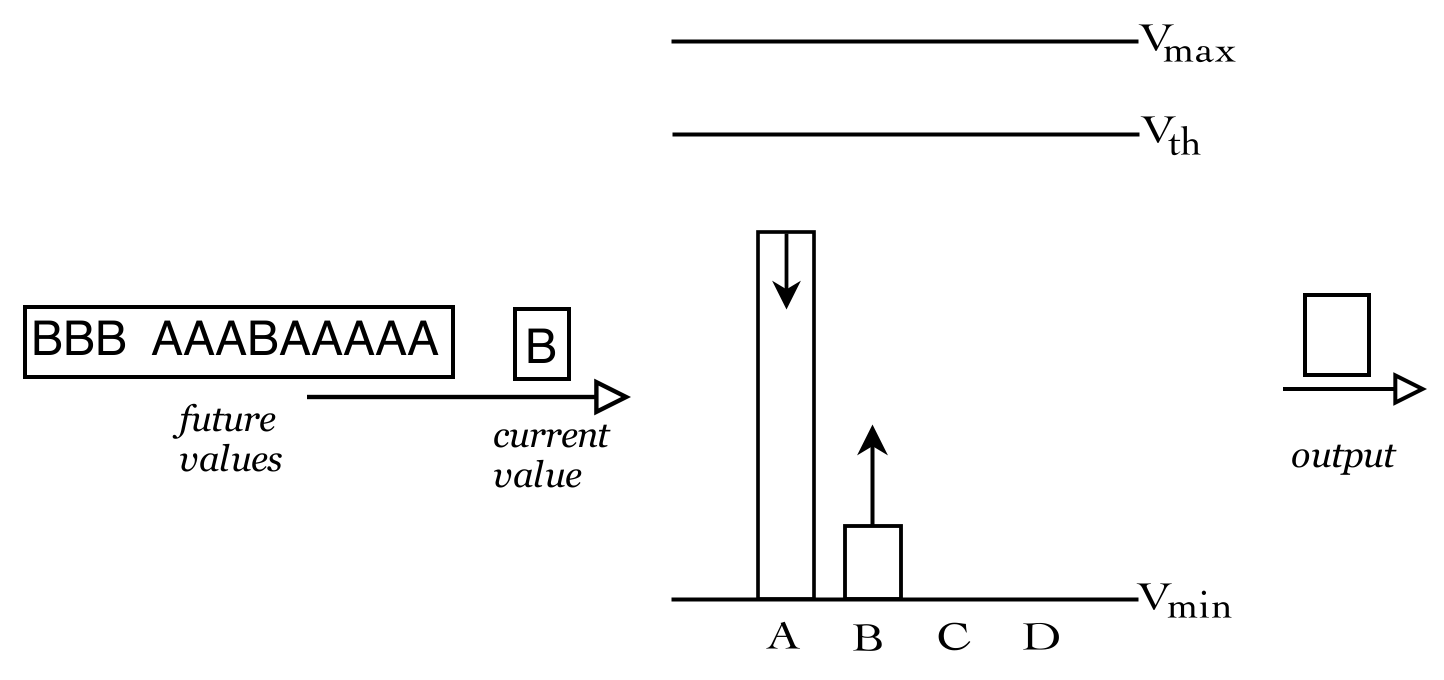
\includegraphics[width=0.7\textwidth]{figures/stabilizer/b.png}
}
\hspace{0.03\linewidth}
\subfloat[B]{
    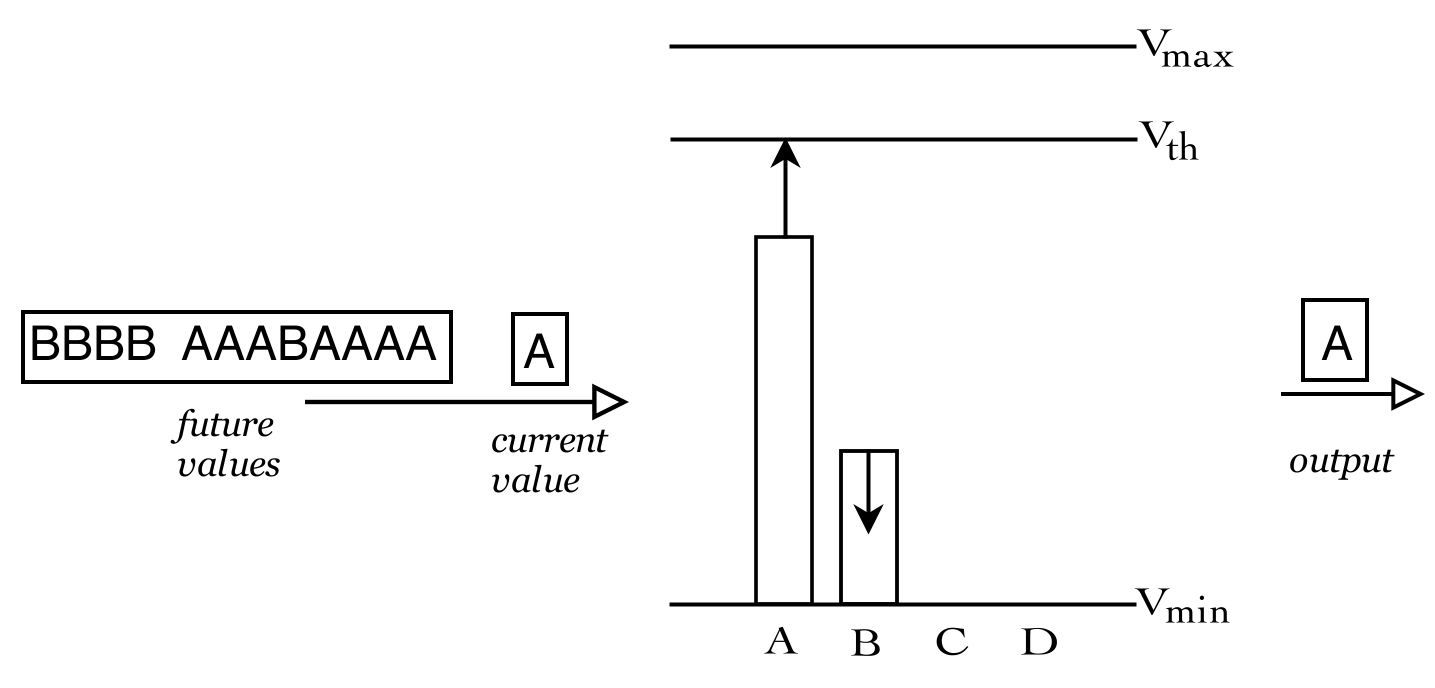
\includegraphics[width=0.7\textwidth]{figures/stabilizer/a.png}
}
  \caption{Two examples of a stabilizer in action}
  \label{fig:stabilizer}
\end{figure}




\subsection*{Training phase}
recording video, manual labeling, extracting HOG features, training classifier

\section{Discussion}
